\documentclass[12pt,a4paper,parskip]{scrreprt}
\usepackage[english,german,ngerman]{babel}
\usepackage[utf8]{inputenc}
\usepackage[T1]{fontenc}
\usepackage{amsmath}
\usepackage{amsfonts}
\usepackage{amssymb}
%http://www.namsu.de/Extra/pakete/Setspace.html
\usepackage{setspace}
%Fußnoten werden das ganze Dokument über durchgezählt
%Quelle: http://golatex.de/nummerierung-der-fussnoten-durchgehend-im-gesamten-dokument-t2042.html
\usepackage{chngcntr}
\counterwithout{footnote}{chapter}
\usepackage{makeidx}
\makeindex
\usepackage{graphicx}
%Für Quellcodeschnippsel
%Für Bash Code Highlighting
\usepackage{minted}
%Anleitung: https://en.wikibooks.org/wiki/LaTeX/Source_Code_Listings
\usepackage{listings}
\usepackage{color}

\definecolor{mygreen}{rgb}{0,0.6,0}
\definecolor{mygray}{rgb}{0.5,0.5,0.5}
\definecolor{mymauve}{rgb}{0.58,0,0.82}

\lstset{ %
  backgroundcolor=\color{white},   % choose the background color; you must add \usepackage{color} or \usepackage{xcolor}
  basicstyle=\footnotesize,        % the size of the fonts that are used for the code
  breakatwhitespace=false,         % sets if automatic breaks should only happen at whitespace
  breaklines=true,                 % sets automatic line breaking
  captionpos=b,                    % sets the caption-position to bottom
  commentstyle=\color{mygreen},    % comment style
  deletekeywords={...},            % if you want to delete keywords from the given language
  escapeinside={\%*}{*)},          % if you want to add LaTeX within your code
  extendedchars=true,              % lets you use non-ASCII characters; for 8-bits encodings only, does not work with UTF-8
  frame=single,	                   % adds a frame around the code
  keepspaces=true,                 % keeps spaces in text, useful for keeping indentation of code (possibly needs columns=flexible)
  keywordstyle=\color{blue},       % keyword style
  language=Octave,                 % the language of the code
  otherkeywords={*,...},           % if you want to add more keywords to the set
  numbers=left,                    % where to put the line-numbers; possible values are (none, left, right)
  numbersep=5pt,                   % how far the line-numbers are from the code
  numberstyle=\tiny\color{mygray}, % the style that is used for the line-numbers
  rulecolor=\color{black},         % if not set, the frame-color may be changed on line-breaks within not-black text (e.g. comments (green here))
  showspaces=false,                % show spaces everywhere adding particular underscores; it overrides 'showstringspaces'
  showstringspaces=false,          % underline spaces within strings only
  showtabs=false,                  % show tabs within strings adding particular underscores
  stepnumber=1,                    % the step between two line-numbers. If it's 1, each line will be numbered
  stringstyle=\color{mymauve},     % string literal style
  tabsize=2,	                   % sets default tabsize to 2 spaces
  title=\lstname                   % show the filename of files included with \lstinputlisting; also try caption instead of title
}
%Überflüssig, dank Dokumentenklasse scrreprt
\usepackage[left=4.00cm, right=2.00cm, top=4.00cm, bottom=2.00cm]{geometry}
%Glossar anschalten und in TOC aufnehmen und erzeugen
%https://en.wikibooks.org/wiki/LaTeX/Glossary
\usepackage{hyperref} %Klickbare Einträge im Glossar
%\usepackage[toc,acronym]{glossaries}
%\makeglossaries
%\usepackage[nomain,acronym,xindy,toc]{glossaries} % nomain, if you define glossaries in a file, and you use \include{INP-00-glossary}
%http://tex.stackexchange.com/questions/111192/problems-with-xindy-and-glossaries
%\usepackage[nonumberlist,nomain,acronym,toc]{glossaries}
% Acronym muss an erster Stelle stehen, sonst funktioniert die Trennung von Abkürzungsverzeichnis und Glossar nicht
\usepackage[acronym,nonumberlist,toc]{glossaries}
%Glossareinträge
\newglossaryentry{GPLv2}
	{
 	 name=GPLv2,
 	 description={is a programmable machine that receives input,
               stores and manipulates data, and provides
               output in a useful format}
	}
\newglossaryentry{psu}
	{
	name=PSU,
	description={Power Supply Unit, Netzteil},
	plural=PSUs
	}
\newglossaryentry{sla}
	{
	name=SLA,
	description={Service Level Agreement}
	}
%Glossareinträge Ende
%Acronyme
\newacronym{rz}{RZ}{Rechenzentrum}
\newacronym{ram}{RAM}{Random Access Memory}
\newacronym{ca}{CA}{Computer Associates}
\newacronym{fc}{FC}{Fibre Channel}
\newacronym{elk}{ELK}{Elasticsearch - Logstash - Kibana}
\newacronym{it}{IT}{Informationstechnik}
\newacronym{omd}{OMD}{Open Monitoring Distribution}
\newacronym{os}{OS}{Betriebssystem}
\newacronym{etc}{etc.}{etcetera}
\newacronym{itil}{ITIL}{Information Technology Infrastructure Library}
\newacronym{sla}{SLA}{Service Level Agreement}
\newacronym{snmp}{SNMP}{Simple Network Management Protocol}
\newacronym{dv}{DV}{Datenverarbeitung}
\newacronym{bspw}{bspw.}{beispielsweise}
\newacronym{zb}{z.B.}{zum Beispiel}
\newacronym{nrpe}{NRPE}{Nagios Remote Plugin Executor}
\newacronym{san}{SAN}{Storage Area Network}
\newacronym{psu}{PSU}{Power Supply Unit}
\newacronym{rest}{REST}{Representational State Transfer}
\newacronym{api}{API}{Application Programming Interface}
\newacronym{cpu}{CPU}{Central Processing Unit}
\newacronym{itsm}{ITSM}{IT Service Management}
\newacronym{llc}{LLC}{Limited Liability Company}
\newacronym{obs}{OBS}{Open Build Service}
\makeglossaries
%\usepackage{imakeidx}
%Tiefe der Nummerierung ändern, Subsubsection ist Ebene 3
%\setcounter{secnumdepth}{3}
% Bibliothek & Zitierstil
\usepackage[style=authortitle-icomp,backend=biber]{biblatex}
\usepackage[babel,german=guillemets]{csquotes}
%\bibliography{seminararbeit_monitoring.bib} %U.u. deprecated
% Anleitung zu BibLaTEX: http://biblatex.dominik-wassenhoven.de/download/DTK-2_2008-biblatex-Teil1.pdf
\addbibresource{seminararbeit_monitoring.bib}
%So werden URLs im Literaturverzeichnis in eine neue Zeile geschrieben
%Quelle: http://www.golatex.de/biblatex-literaturverzeichnis-zeilenumbruch-vor-url-t8406.html
\DeclareFieldFormat{url}{\newline URL: \url{#1} }
\setuptoc{toc}{bibliography=totoc}
% Abkürzungsverzeichnis mit Nomencl
% siehe http://texwelt.de/wissen/fragen/4942/wie-kann-ich-die-erstellung-eines-abkurzungsverzeichnisses-mit-dem-paket-nomencl-automatisieren
% und http://golatex.de/abkuerzungsverzeichnis-mit-texmaker-t8301.html
% Zum aktualisieren muss "Makeindex" aufgerufen werden, Konfiguration siehe letzter Link
%\usepackage[intoc]{nomencl}
% Befehl umbenennen in abk
%\let\abk\nomenclature
% Überschrift
%\renewcommand{\nomname}{Abkürzungsverzeichnis}
% Punkte zw. Abkürzung und Erklärung
%\setlength{\nomlabelwidth}{.20\hsize}
%\renewcommand{\nomlabel}[1]{#1 \dotfill}
% Zeilenabstände verkleinern
%\setlength{\nomitemsep}{-\parsep}
%\makenomenclature
% Ende Abkürzungsverzeichnis





\begin{document}
	%TODO: Titelseite an die Erfordernisse anpassen
	%http://golatex.de/wiki/Widmung
	\subject{Seminararbeit im Studiengang \glqq Verwaltungsinformatik\grqq}
	\author{Markus Österle}
	\title{Servermonitoring in Rechenzentren}
	\subtitle{am Beispiel von Linux Systemen}
	\publishers{Betreut von Dipl. Inf. Stefan Müller}
	\date{} % setzt ein leeres Datum und löscht quasi das per default verwendete \today von der Titelseite

	\maketitle
	\setcounter{tocdepth}{3}
	\tableofcontents
	% Gibt das Latex Logo aus...Stelle? 
	%\LaTeXe{}
%Ab hier 1.5facher Zeilenabstand 
	\onehalfspacing
	\chapter{Einleitung}
Das Thema des Servermonitorings hat sich im professionellen \acrshort{rz} Umfeld in den letzten Jahren zu einem großen Thema entwickelt. Durch die steigende Komplexität der Systeme steigen auch die Anforderungen an die Überwachung der selbigen, reichte es in den 90er Jahren noch aus von einem zentralen Rechner (gemeint ist hier ein normaler Personal Computer) per Ping zu Überwachen ob Rechner verfügbar sind, so wird heute ein sehr viel feineres Monitoring erwartet. Nicht nur die Erreichbarkeit der Rechner soll überwacht und statistisch aufbereitet werden, sondern auch die Auslastung und die Gesundheit einzelner Bauteile (bspw. \gls{psu}, \acrshort{ram} Bausteine). 

In der vorliegenden Arbeit wird das Thema und die Historie des Servermonitorings unter Begrenzung auf das Teilgebiet Linux-Systeme betrachtet. Dies hat zum einen den Grund, dass der Autor viele Jahre Erfahrung mit Linux und Unix Betriebssystemen vorweisen kann und schon einige Erfahrung mit der Überwachung von *nix-Servern gemacht hat.
	\section{Warum Monitoring im Rechenzentrum?}
	%TODO kritische Betriebszustände definieren?
	Aus der Systemadministratorensicht macht es eigentlich von Grunde auf Sinn soviele Informationen wie nur möglich über seine Systeme zu haben, dies macht es zum einen möglich schnell auf kritische Betriebszustände zu erkennen und zu beheben. Zum anderen um gegenüber der Führungsebene Material für eventuelle Rechtfertigungen zu haben am besten grafisch aufbereitet und selbsterklärend.
	
		Überwachung der Serverauslastung
		
		Proaktive Erkennung von (Hardware)Defekten
		
		\gls{sla} Überwachung
	\section{Warum Linux?}
	Systemüberwachung ist natürlich für alle Komponenten im Rechenzentrum wichtig, begonnen bei der Basisversorgung (Strom, Kühlung) über die grundlegende Infrastruktur (Netzwerkinfrastruktur, evtl. Storageinfrastruktur)bis zu den einzelnen Systemen (natürlich quer über die Betriebssystemgrenzen hinweg). Mit den später in dieser Arbeit vorgestellten Lösungen können viele dieser Felder abgedeckt werden, eine genaue Beschreibung des wie würde allerdings den (sowohl den zeitlichen als auch den mengenmäßigen) Rahmen der Arbeit sprengen. Deshalb werden wir uns in der Folge auf das Thema der Serverüberwachung von Linux Systemen spezialisieren. Für Linux spricht auch, dass es zum einen eine relativ große Verbreitung im Serverbereich hat und die Arbeit auch für den privaten Gebrauch nicht irrelevant ist, da der Überwachung mit den vorgestellten Tools keine Grenzen gesetzt sind durch den modularen Aufbau und die Erweiterbarkeit mit selbstgeschriebenen Skripten, Plugins, \acrshort{etc}. sind der Phantasie keine Grenzen gesetzt. Die Systeme können beispielsweise ohne großen Aufwand und geistige Eigenleistung (Anleitungen und Code für vieles gibt es bereits im Netz) für die Überwachung privater Webservices, privater Netzwerkinfrastrukturen, SmartHomes, Wetterstationen, \acrshort{etc} genutzt werden.
	%TODO Verbreitung von Linux im Serverbereich Grafik und Quelle
		
	
	\chapter{Vom Ping zum proaktiven Monitoring}
	In den folgenden Unterkapiteln werde ich mich mit der grundlegenden Definition von Begriffen rund um das Thema Monitoring/Serverüberwachung beschäftigen und einen kleinen Überblick über die Historie geben.
	\section{Historie}
	große Maschinen die alle Software gebündelt hatten und einfacher zu überwachen waren
	Zersplitterung der Software auf viele kleinere Maschinen, dadurch erhöhter Überwachungsaufwand, zusärtlich auch gestiegene Anforderungen an Verfügbarkeit und damit auch an eben dieses Monitoring.
	Top und seine Derivate, SAR Daten (Sysstat) die aber erst vom Server geholt und grafisch (KSar) aufbereitet werden müssen. Systemlogs die in ihrer Vielzahl unüberblickbar sind und um Sie überhaupt verarbeiten zu können auf jeden Fall gefiltert und aufbereitet werden müssen. Auch eine zunehmende Standardisierung der IT Prozesse wie beispielsweise \gls{itil}\ (\glsdesc{itil}) tragen ihren Teil zur Notwendigkeit von immer umfangreicheren Monitoring und Reportingsystemen bei.
	\subsection{ITIL die Quelle allen Übels?}
	Definition ITIL - ITIL \& Monitoring?
	Definition SLA
	Definition Servicelevel
	Was verbirgt sich nun hinter magischen Begriffen wie \gls{itil} und Monitoring, in der folge werde ich versuchen die gebräuchlichsten Definitionen darzulegen und zu beschreiben wie die einzelnen Spielarten des Monitorings mittels Tools im praktischen Teil der Arbeit umgesetzt werden.
	\section{Definition (Server-/System-)Monitoring}
	\subsection{Allgemein}
	%TODO Definition Monitoring
	Laut dem Duden handelt sich beim Monitoring um
	\begin{center}
		\glqq[Dauer]beobachtung (eines bestehenden Systems)\grqq\footcite[S. 701; Stichwort Monitoring]{duden}
	\end{center}
	Dieser Definition ist auch aus Informatikersicht nicht mehr allzuviel hinzuzufügen, außer dass es sich natürlich in unserem Fall um die Beobachtung eines \acrshort{it}-Systems handelt.
	\subsection{proaktives Monitoring}
	%http://www.thefreedictionary.com/proactive
	Unter \glqq proaktiv\grqq\ versteht man 
	Unter \glqq proaktivem Monitoring\grqq\ versteht man bei ITIL: \glqq Das proaktive Monitoring in seiner Überwachung achtet auf bestimmte Verhaltensmuster (Patterns), um künftige Ausfälle vorauszusehen. \grqq\ 
	Notwendig möglichst viele Informationen zu haben um Muster erkennen zu können.
	\subsection{reaktives Monitoring}
	\subsection{Verfügbarkeitsmonitoring}
	Historie
	\subsection{SLA Monitoring}
	Einhaltung vereinbarter Servicelevel \footcite[40]{iso20000sla}
	\subsection{Fazit}
	Um alle in den vergangenen Unterkapiteln beschriebenen Anforderungen zu erfüllen ist es notwendig mehrere Überwachungstechnologien zu verbinden, um ein optimales Monitoring zu erhalten. So ist es zur proaktiven Erkennung von Fehlern zum einen unerlässlich die Einträge in Logfiles auswerten zu können, um Fehler zu bemerken lange bevor Sie beginnen sich auf den Produktivbetrieb auszuwirken (bspw. Schreibfehler auf ein per \acrlong{fc} (\acrshort{fc}) angebundenes \gls{san}-System oder einfach I/O Fehler auf eine der Systemfestplatten) und zum anderen auch die Performance der Systeme im Auge zu behalten um sicher zu stellen, dass die Dimensionierung der Systeme richtig ist und nicht plötzliche Engpässe auftreten können.
	\chapter{Monitoring Systeme für Linux Server}
	Wenn man zu dem Thema \glqq Monitoringsysteme für Linux\grqq\ im Internet recherchiert wird man neben den diversen teuren Softwarelösungen diverser Hersteller immer wieder über einen Namen stolpern: Nagios. Das Tool hat sich fürs Monitoring von Linux Systemen zu einer Art Industrie Standard entwickelt. Das mag zum einen an seiner freien Verfügbarkeit liegen, zum anderen aber vielleicht auch daran, dass im Linux Umfeld viele Administratoren die Quelloffenheit und die leichte Erweiterbarkeit mittels eigener Tools, Plugins, Agenten von Nagios schätzen. Darüber hinaus findet man ein weites Angebot an Support und Serviceleistungen, sowohl im Internet, als auch von Consultingfirmen, die meist auch an der Entwicklung der Systeme beteiligt sind.
	
	
	\section{Performance \& SLA Monitoring}
	%TODO: Warum Check_MK, warum nicht OMD, Vielfalt der Systeme OMD, Check_MK, OMD Lab Edition, bei ursprünglicher OMD auf der Seite nichts passiert, hinter den Kulissen aber schon, warum empfiehlt es sich trotzdem über eine Subskription nachzudenken (Förderung OS Gedanken, Professionieller Support und Schulung, mehr Features die erst später irgendwann in der freien Version ankommen)
	\subsection{Nagios}
	%TODO: Nagios als Kern, mit wenigen zusätzlichen Funktionen, die Funktionsumfänge die wir in der großen Version sehen werden mit externen Programmen realisiert.
	\begin{figure}
	\centering
	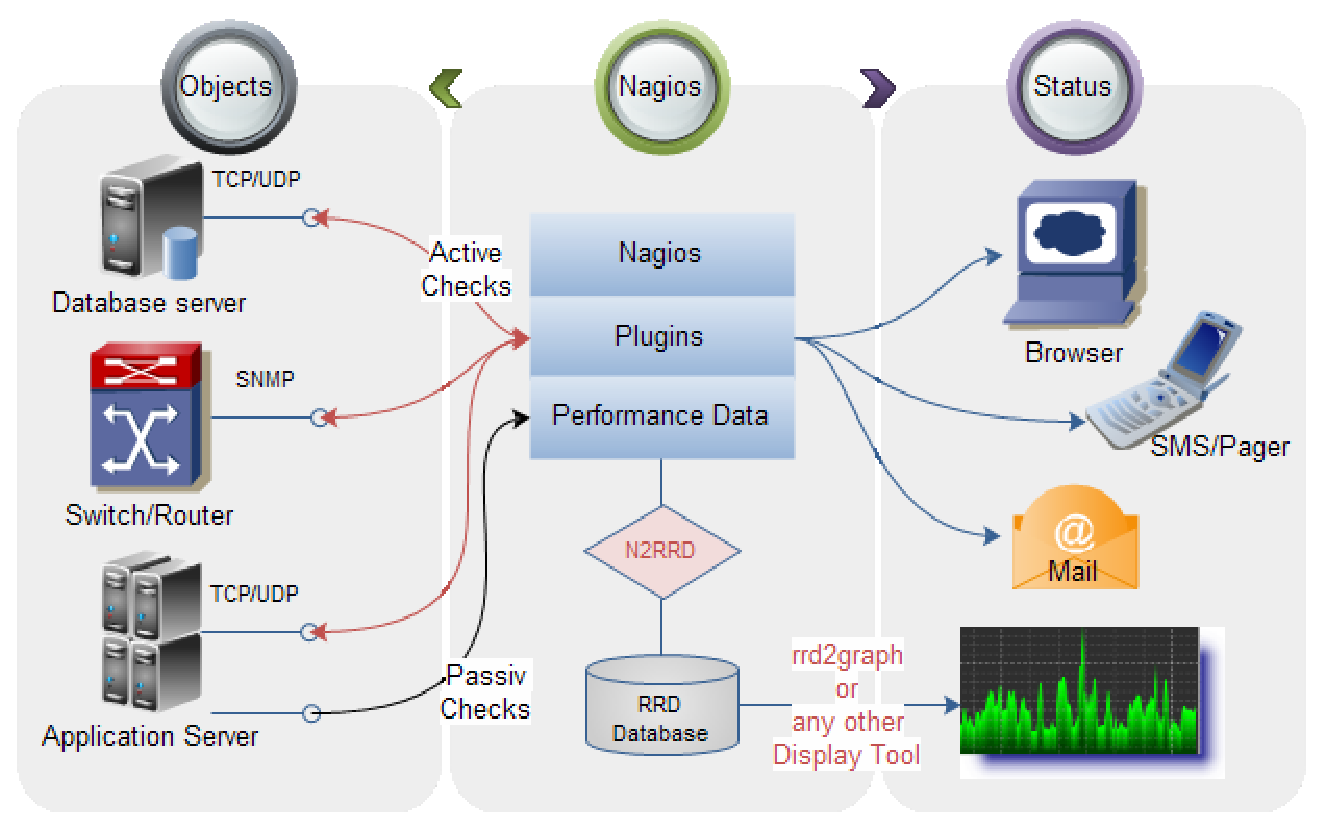
\includegraphics[width=1\textwidth]{pics/NagiosMonitoring.eps}
    \caption[Grober Aufbau von Nagios]{Aufbau einer Nagios Appliance (Quelle: „Monitoring“ von Diglinks in der Wikipedia auf Englisch - Übertragen aus en.wikipedia nach Commons durch Esquilo.. Lizenziert unter Gemeinfrei über Wikimedia Commons - https://commons.wikimedia.org/wiki/File:Monitoring.png\#/media/File:Monitoring.png)}
	\end{figure}
	\begin{figure}
		\centering
		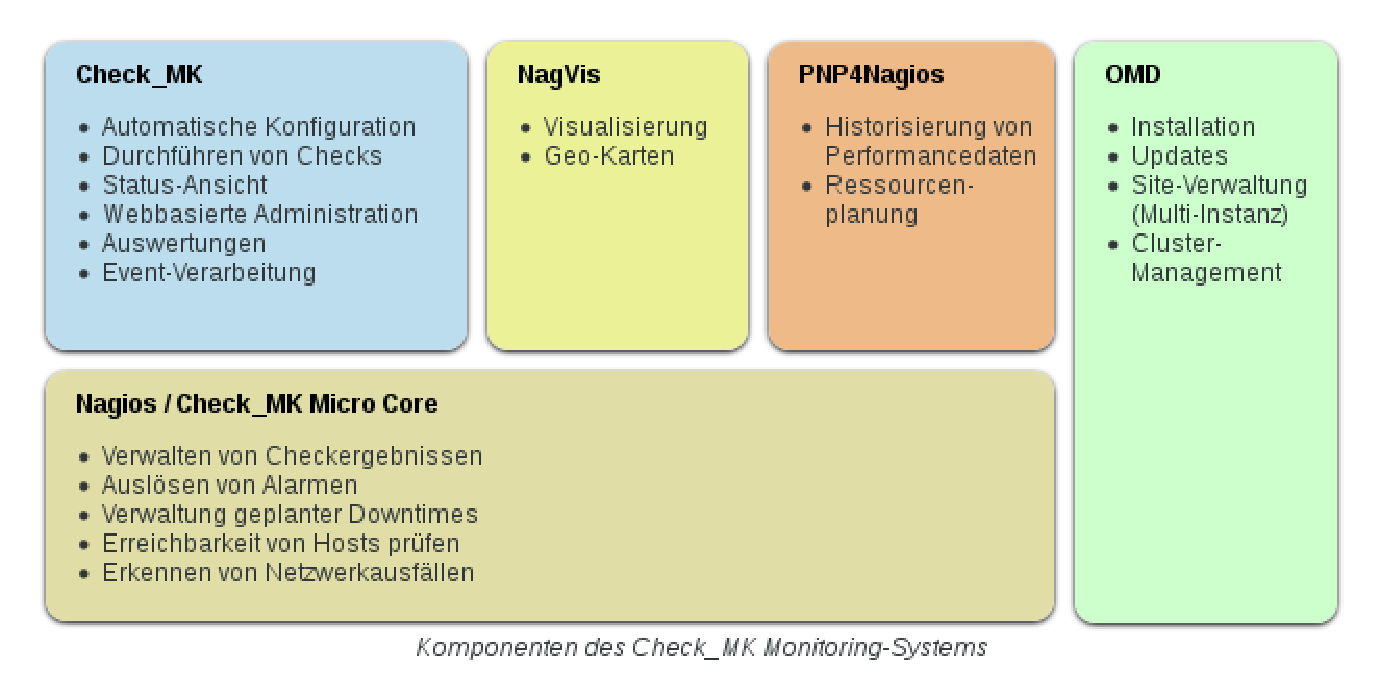
\includegraphics[width=1\textwidth]{pics/checkMKAufbau.eps}
		\caption[Komponenten des Check\_MK Monitoring Systems]{Komponenten des Check\_MK Monitoring Systems (Quelle: \cite{checkmkmonitoringpic})}
	\end{figure}
	\begin{figure}
	\centering
	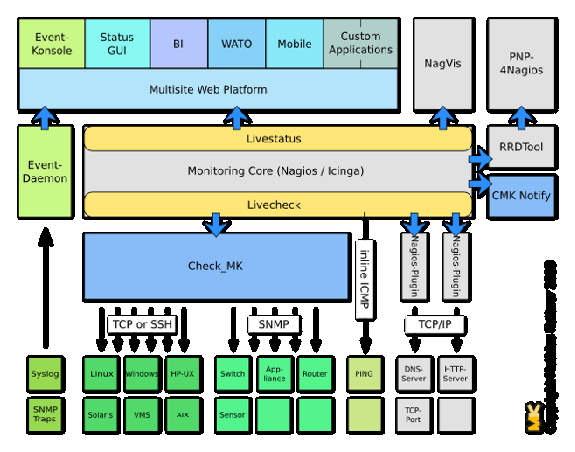
\includegraphics[width=1\textwidth]{pics/OMD_Schema.eps}
    \caption[Aufbau von Check\_MK]{Aufbau von Check\_MK (Quelle: \cite{checkmk})}
	\end{figure}
	\subsubsection{Historie}
	Der Name Nagios ist wie viele Namen im Linux Umfeld ein rekursives Akronym. Das sich herleitet aus dem initialen Namen des Projekts \glqq Netsaint \grqq\ der aus rechtlichen Gründen im Jahr 2002 in Nagios geändert wurde. 
	\footcite{nagioshistory} \footcite{nagiosnamefaq}
	
	Nagios -> Kritik Weiterentwicklung Ethan Galstedt...siehe Lehrgangsunterlagen QSkills
	Icinga, Shinken
	check\_mk als Bundle Lösung die verschiedene Backends bereithält, inkl. mittlerweilen eigenem Backend (Microkernel)
	Fertige Lösung im Bundle mit mehr Tools
	OMD -> checkmk Änderung im Subskriptionsmodell
	check\_mk Versionen Freie Version, Subskriptionen: Innovation, Stable, etc.
	
	\subsubsection{Lizenzmodell}
	Erläuterung GPLv2 \footcite{gplv2de}\footcite{gplv2en}
	\gls{GPLv2}
	\subsubsection{Funktionsumfang}
	
	\section{Logfile Monitoring}
	\subsection{Syslog-ng und Rsyslog}
	Der erste Gedanke fällt hierbei auf die in den bisherigen BS Vorlesungen gelernten Technologien, weshalb ich hier von dem Schema ein Tool aus der offenen und eines aus der kommerziellen Welt abweichen möchte.
	Problematisch in nicht homogenen Umgebungen mit verschiedenen Versionen aktueller Distributionen, weil systemd...ELK Stack ist hier besser weil vielseitiger
	\footcite{systemd2015}
	%\subsection{Splunk Monitoring}
	\subsection{Elasticsearch - Logstash - Kibana}
	Oftmals auch \acrshort{elk} oder ELK-Stack genannt sind eigentlich die drei voneinander unabhängige Tools \acrlong{elk}.
	\subsubsection{Elasticsearch}
	\subsubsection{Logstash}
	\subsubsection{Kibana}
	\chapter{Praktische Vorstellung der Funktionalität eines Monitoring Systems}
	\section{Versuchsaufbau}
	Um kurz noch einen praktischen Einblick in die verwendete Software zu geben wird sich der folgende Teil mit dem praktischen Aufbau einer kleinen \glqq Spielwiese\grqq beschäftigen. Im wesentlichen besteht dieser Aufbau aus zwei virtuellen Maschinen die mittels VirtualBox realisiert wurden und einem entfernten Server der bei einem großen Hoster in einem Rechenzentrum steht.
	\subsection{verwendete Software}
	Opensuse Leap 42.1 als Betriebssystem für den Überwachungsrechner auf dem sowohl die Check\_MK Instanz läuft, als auch der ELK Stack. Der entfernte Rechner der per check\_by\_ssh abgefragt wird ist ein virtueller Server bei einem großen Hoster, als Betriebssystem läuft auf diesem Rechner Opensuse 13.2 (64bit) mit der für Webserver üblichen Software (LAMP-Stack = Linux Apache Mysql PHP) und zusätzliche zwei Java Anwendungen (Jenkins \& Sonarqube). An zusätzlicher überwachter Sicherheitssoftware ist Fail2Ban installiert und so konfiguriert, dass Hosts die 3 fehlerhafte Versuche sich per SSH einzuloggen unternehmen automatisch für eine bestimmte Zeit auf eine Sperrliste in der Firewall gesetzt werden. \\
	\begin{table}[h] %Quelle: http://www.weinelt.de/latex/table.html
	\begin{center}
	\begin{tabular}{|c|c|c|}
	\hline 
	Eingesetzte Software & Version & Client oder Server \\ 
	\hline 
	VirtualBox & 5.0.10 & Virtualisierungslösung\\
	\hline
	Opensuse & 13.2 & Server\\ 
	\hline 
	Opensuse & Leap 42.1 & Client\\
	\hline
	Apache & 2.4 & Server\\
	\hline
	\acrshort{omd} & 2.11.20160108-labs-edition & Server\\
	\hline
	\end{tabular} 
	\caption[Eingesetzte Softwareversionen]{Für den praktischen Teil der Arbeit eingesetzte Softwareversionen mit ihrem Einsatzort}
	\end{center}
	\end{table}
	\subsection{Installation}
	Um die Software und eventuelle Aktualisierungen permanent verfügbar zu haben, empfiehlt es sich das angebotene Repository \footcite{omdrepo} einzubinden, beim verwendeten OpenSuse funktioniert das wie in Listing 4.1 Zeile 1 gezeigt. Anschließend muss die Software mitsamt ihren Abhängigkeiten installiert werden, dies wird mittels des Paketmanagers \textit{zypper} mit dem wir eben schon das Repository eingehängt haben realisiert (Listing 4.1, Zeile 2). Nach dem Abschluß der Paketinstallationen ist die \acrshort{omd} einsatzbereit.
	\begin{lstlisting}[language=bash, caption=Konfiguration eines Repositories und Installation der \acrfull{omd}]
	zypper ar -f https://labs.consol.de/repo/testing/sles12/consol-labs.repo
	zypper in omd
	
	wget https://mathias-kettner.de/support/1.2.6p15/check-mk-raw-1.2.6p15-sles12-34.x86_64.rpm
	zypper in check-mk-raw-1.2.6p15-sles12-34.x86_64.rpm
	omd setup
	\end{lstlisting}
	\subsection{Konfiguration}
	
	\section{Performancemonitoring}
	\subsection{Überwachung eines entfernten Servers}
	\begin{lstlisting}[language=bash]
	root@linux# ssh -i check_mk.key targethost
	\end{lstlisting} \footcite{checkmkCheckBySSH2015}
	\subsection{Überwachung einer Datenbank}
	\section{Service Level Agreement Monitoring}
	%TODO Beschreibung anhand der Verfügbarkeit einer Webseite
	\subsection{Überwachung der Verfügbarkeit einer Datenbank}
	MySQL DB und Derby als Beispiel für die Überwachung einer in Memory Datenbank.
	\subsection{Überwachung der Verfügbarkeit einer Webseite}
	\section{Logfile Monitoring}
	
	% Abkürzungsverzeichnis auf einer neuen Seite ausgeben
	%\printnomenclature
	% Literaturverzeichnis ausgeben und als Eintrag gleichwertig mit einem Kapitel ins Inhaltsverzeichnis eintragen
	\begingroup
	\nocite{*} %Alle Einträge des Literaturverzeichnisses auch ohne Zitierung ausgeben
	\printbibliography 
	\addchaptertocentry{}{Literatur}
	%\addcontentsline{toc}{chapter}{Literatur}
	\endgroup
	\printglossary[title=Abkürzungsverzeichnis, type=\acronymtype] % prints just the list of acronyms	
	\printglossary[title=Glossar]
	%\printglossaries	
	\listoffigures % Abbildungsverzeichnis
	\addchaptertocentry{}{Abbildungsverzeichnis}
	\listoftables % Verzeichnis der Tabellen
	\addchaptertocentry{}{Tabellenverzeichnis}
\end{document}